\section{System Overview}

\subsection{System Concept}
After reviewing the requirements and doing the necessary research,
a established simple use case was created to illustrate the system concept as in figure \ref{fig:usecase}.

\begin{figure}[h]
    \centering
    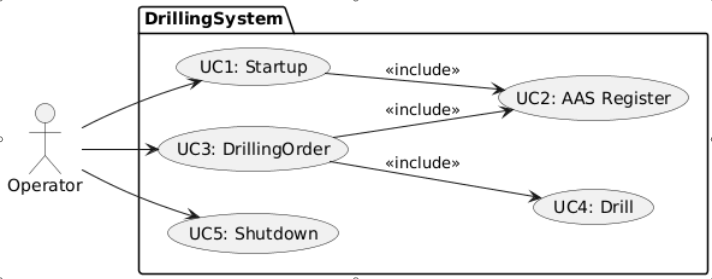
\includegraphics[width=0.8\textwidth]{Images/Usecase.png}
    \caption{System Use Case}
    \label{fig:usecase}
\end{figure}

From the use case and the requirements, the system concept is established where it holds two
main components:
\begin{itemize}
    \item \textbf{An Asset Administration Shell (AAS)}
    \item \textbf{A Run time Environment (RTE) with Multiagent System (MAS)}
\end{itemize}
\begin{figure}[h]
    \centering
    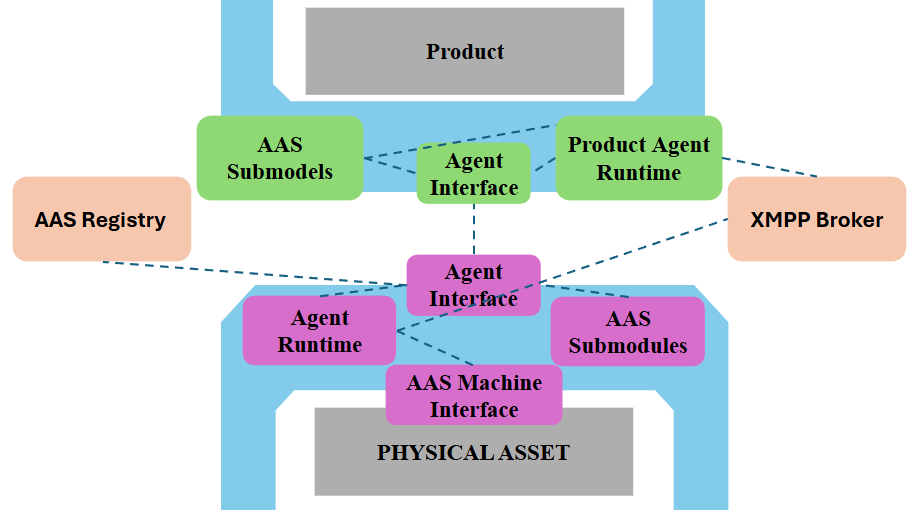
\includegraphics[width=0.8\textwidth]{Images/System_Concept.png}
    \caption{System Concept}
    \label{fig:system_concept}
\end{figure}

The Concept illustrated in figure \ref{fig:system_concept} shows the two main parts , the Product or Production AAS and the Resource AAS.

\subsection{Resource AAS - Overview}
The Resource AAS is the component that describes a resource in the System,
where a Resource in the system can vary from a simple machine to a worker.
The Resource AAS contains the following components:
\begin{itemize}
    \item \textbf{AAS Submodels} that describe the resource properties and capabilities.
    \item \textbf{Agent Runtime} that contains the agent that represents the resource in the system.
    \item \textbf{AgentInterface} that connects the resource Agent to other agents in the system.
    \item \textbf{Agent Machine Interface} that connects the resource Agent to the machine or worker it represents.
\end{itemize}

The Submodels of the Resource AAS contains the following components as in table \ref{table:resource_aas_submodels}.

\begin{table}[h]
\centering
\begin{tabularx}{\textwidth}{>{\raggedright\arraybackslash}X>{\raggedright\arraybackslash}X}
\toprule
\rowcolor[HTML]{38FFF8}
\textbf{Submodel} & \textbf{Description} \\ \midrule
\textbf{Operation State Submodel} & Contains the current operational state of the resource and History. \\
\textbf{Knowledge Submodel} & Contains the knowledge of the resource constraints and the environmental conditions. \\
\textbf{Capabilities Submodel} & Describes the skills the asset can perform and the services it can provide. \\
\textbf{Interaction and scheduling Submodel} & Contains the Communication endpoints and the collaboration mechanisms. \\
\bottomrule
\end{tabularx}
\caption{Resource Agent : Submodels}
\label{table:resource_aas_submodels}
\end{table}
The submodels then could provide the necessary information for the Resource Agent to perform its tasks in the system.
The Resource Agent then connects to other agents in the system through the Agent Interface and to the machine.
As shown in figure \ref{fig:resource_aas_overview}. the Belifes of the agent are updated from the
operational state submodel and the knowledge submodel where they provided the necessary state and constraints for the agent.
The Desires of the agent are established from the capabilities submodel
where they provide the skills and services.
Finaly the agent can act upon the desiers and excute its intention which the scheduling and interaction submodel
can provide the necessary information for the agent to interact and schedule its tasks.
\begin{figure}[h]
    \centering
    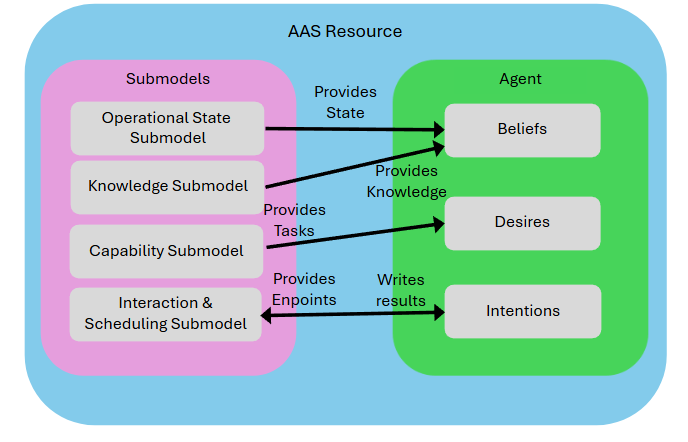
\includegraphics[width=0.8\textwidth]{Images/Resource_Agent_overview.png}
    \caption{Resource AAS Overview}
    \label{fig:resource_aas_overview}
\end{figure}

\newpage
The Resource AAS can interact with other AASs (production or resource).
It also capable of publishing events and subscribing to other AAS events.
As shown in figure \ref{fig:resource_aas_interactions}, the Resource AAS can interact with other AASs through
via XMPP protocol which is a communication protocol for MAS frame work for python \textbf{SPADE}.
XMPP can also be used as a broker for the AAS to publish and subscribe to events.
Finaly the Resource AAS can interact with the Asset via a custom Interface (OPC UA, REST API ...etc).
\begin{figure}[h]
    \centering
    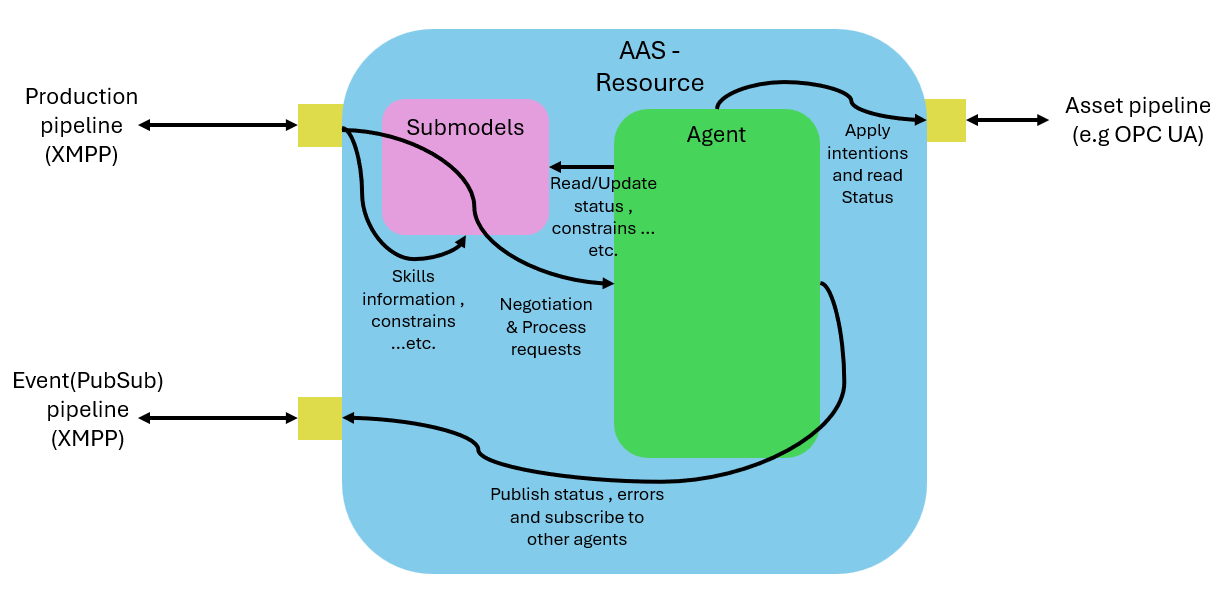
\includegraphics[width=0.99\textwidth]{Images/Resource_Agent_Interaction_Overview.png}
    \caption{Resource AAS Interactions - Overview}
    \label{fig:resource_aas_interactions}
\end{figure}
The communication interfaces and their usage are summarized in table \ref{table:communication_interfaces}.
\begin{table}[h]
\centering
\begin{tabularx}{\textwidth}{>{\raggedright\arraybackslash}X>{\raggedright\arraybackslash}X}
\toprule
\rowcolor[HTML]{38FFF8}
\textbf{Communication Interface} & \textbf{Usage} \\ \midrule
XMPP & Agent-to-agent communication within the MAS framework. \\
XMPP - Events & Publishing and subscribing to events between AASs. \\
Asset Interface (e.g OPC UA) & Interfacing with industrial assets and machines for data exchange and control. \\
\bottomrule
\end{tabularx}
\caption{Communication Interfaces and Their Usage}
\label{table:communication_interfaces}
\end{table}
\newpage
Internally the Submodels are connected to the agent where they could be read and updated.
The Submodels can also provide the production agents with the available services and skills the resource can provide and the state of the resource.
The Agent runtime can connect to the other agents in two ways:
\begin{itemize}
    \item \textbf{Direct Communication} where the agents can communicate directly with each other and hold negotiations.
    \item \textbf{Event-based Communication} where the agents can publish and subscribe to events.
\end{itemize}
Also it handles the execution of the tasks on the machine or worker it represents.

\newpage
\subsubsection{Resource AAS - Architecture Overview }

\begin{figure}[h]
    \centering
    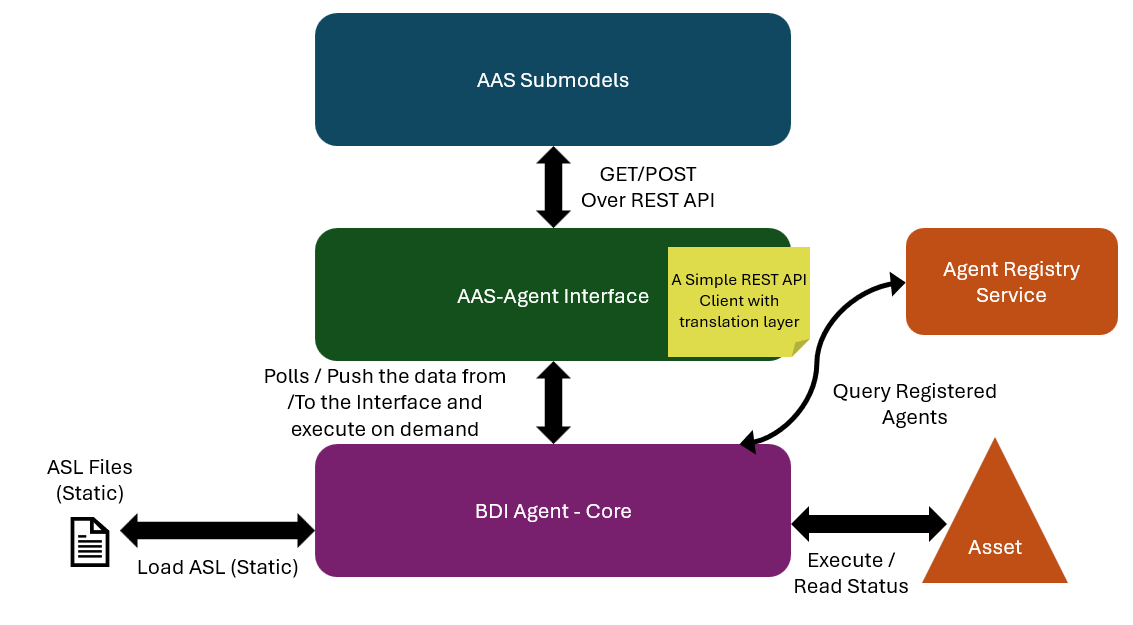
\includegraphics[width=0.99\textwidth]{Images/Resource_Agent_Arch_overview.png}
    \caption{Resource AAS Architecture Overview}
    \label{fig:resource_aas_architecture_overview}
\end{figure}
From an Architecture point of view the Resource AAS can be illustrated as in figure \ref{fig:resource_aas_architecture_overview}.
The overview of the architecture shows three main layers, The \textbf{AAS Submodels} , \textbf{The AAS - Agebnt Interface} and Finaly \textbf{BDI Agent Core}.
The AAS Submodels layer are created via \textbf{Basyx} framework which is an open source framework for creating AASs.
This framework provides the necessary tools to create and manage AASs and their submodels.
It also can provide a REST API for the AAS to be accessed and managed.
The AAS - Agent Interface layer is responsible for connecting the AAS to the Agent Core.
It mainly work as a middleman between the AAS and the Agent Core where it translate the data types of from and to the AAS and the Agent Core.
Finaly The BDI Agent Core is the main component of the Resource AAS where it contains the BDI agent that represents the resource in the system.
The BDI agent is created via \textbf{SPADE} framework which is an open source framework for creating Multi-agent systems in python.
The BDI agent is responsible for managing the beliefs, desires and intentions of the agent.
It also handles the communication with other agents in the system via XMPP protocol.
The BDI agent can also execute the tasks on the machine or worker it represents.
The BDI agent also can register itself with a Agent Registry service that the production Agents
use for discovering the available resources in the system.

\newpage
\subsubsubsection{Submodels with REST API and server}
\begin{figure}[h]
    \centering
    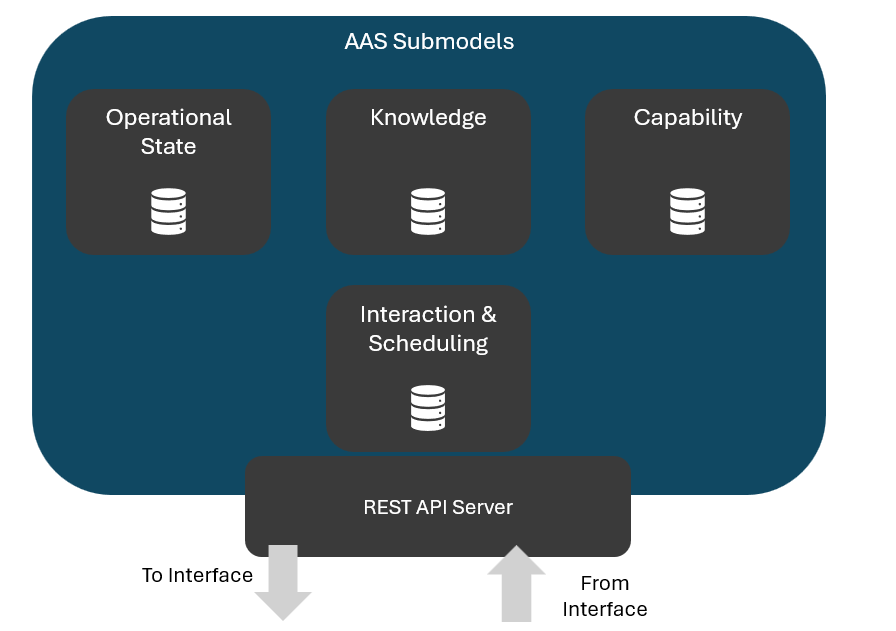
\includegraphics[width=0.8\textwidth]{Images/Resource_Agent_Submodels_Arch_Overview.png}
    \caption{Resource AAS Submodels with REST API and Server}
    \label{fig:resource_aas_submodels_rest_api}
\end{figure}

The Submodels layer as shown in figure \ref{fig:resource_aas_submodels_rest_api} contains the AAS Submodels and a REST API server.
The AAS Submodels are created via \textbf{Basyx} framework which is an open source framework for creating AASs.
This framework provides the necessary tools to create and manage AASs and their submodels.
It also can provide a REST API for the AAS to be accessed and managed.
The Submodels connects to the AAS-Agent Interface via REST API calls where the AAS-Agent Interface can read and update the submodels.

\newpage
\subsubsubsection{AAS-Agent Interface}
\begin{figure}[h]
    \centering
    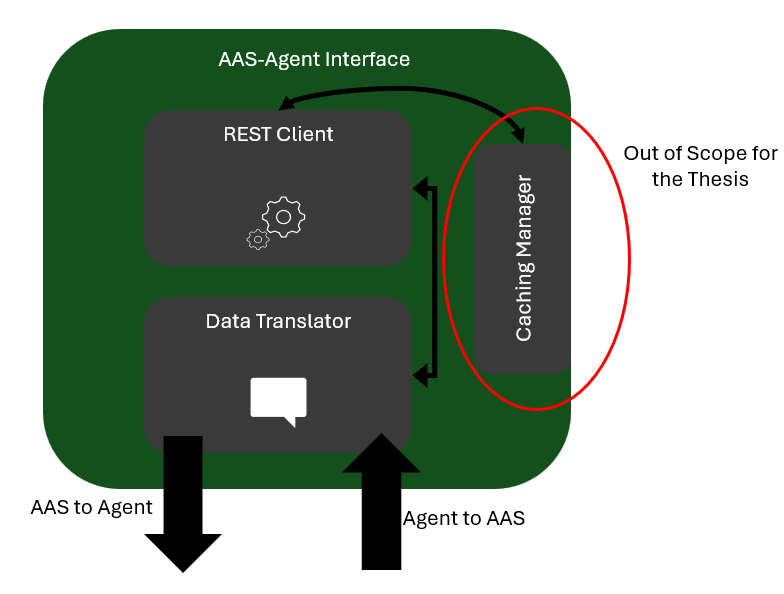
\includegraphics[width=0.9\textwidth]{Images/Resource_Agent_AAS_Agent_interface.png}
    \caption{Resource AAS-Agent Interface}
    \label{fig:resource_aas_agent_interface}
\end{figure}
\\
As in figure \ref{fig:resource_aas_agent_interface} the AAS-Agent Interface is responsible for connecting the AAS to the Agent Core.
It mainly work as a middleman between the AAS and the Agent Core where it translate the data types of from and to the AAS and the Agent Core.
The AAS-Agent Interface contains the following components:
\begin{itemize}
    \item \textbf{REST Client} that connects to the AAS via REST API calls.
    \item \textbf{Data Translator} that translates the data types from and to the AAS and the Agent Core.
\end{itemize}

\newpage
\subsubsubsection{BDI Agent Core}
\begin{figure}[h]
    \centering
    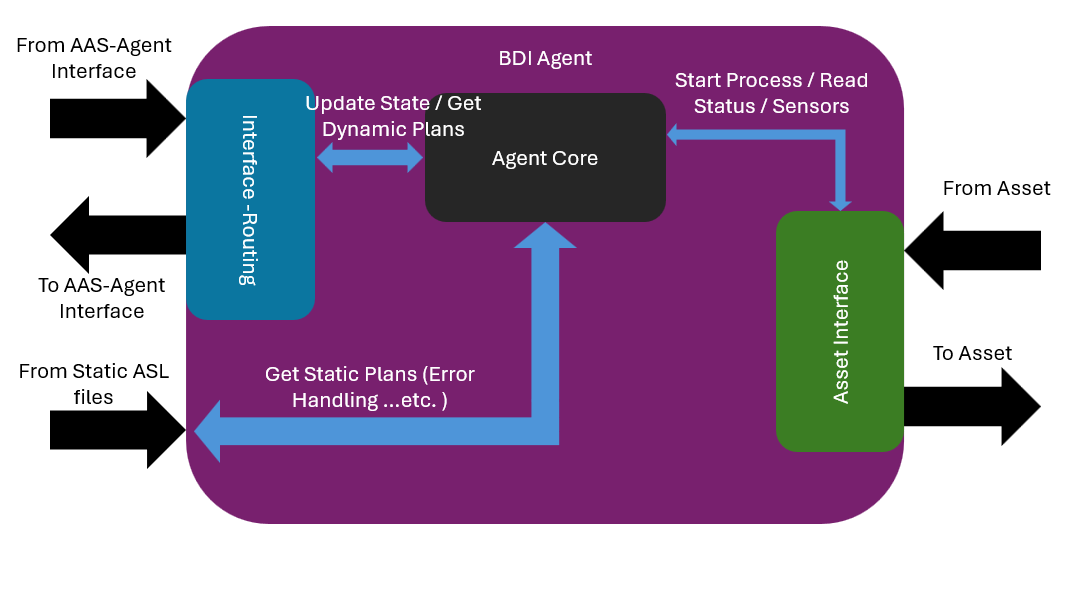
\includegraphics[width=0.99\textwidth]{Images/Resource_Agent_BDI_Overview.png}
    \caption{Resource AAS - BDI Agent Core}
    \label{fig:resource_aas_bdi_agent_core}
\end{figure}
\\
As in figure \ref{fig:resource_aas_bdi_agent_core} the BDI Agent Core is the main component of the Resource AAS where it contains the BDI agent that represents the resource in the system.
The BDI agent is created via \textbf{SPADE} framework which is an open source framework for creating Multi-agent systems in python.
The BDI agent is responsible for managing the beliefs, desires and intentions of the agent.
It also handles the communication with other agents in the system via XMPP protocol.
The BDI agent can also execute the tasks on the machine or worker it represents.
The BDI agent also can register itself with a Agent Registry service that the production Agents
use for discovering the available resources in the system.
The BDI agent contains the following components:
\begin{itemize}
    \item \textbf{Agent Core} that contains the BDI agent and its components.
    \item \textbf{Asset Interface} that connects the agent to the machine or worker it represents.
\end{itemize}
The Agent Core connects with the AAS-Agent Interface so that it can read and update the AAS Submodels.
The Agent Core also connects to other agents in the system via XMPP protocol.
The Agent Core can delegate tasks to the Asset Interface so that it can execute the tasks on the machine or worker it represents.
The Asset Interface connects to the machine or worker via a custom interface (e.g OPC UA, REST API ...etc).

\newpage
\subsection{Production AAS - Overview}

The Production AAS is the component that describes a product in the System,
where a Product in the system can vary from a simple product to a complex assembly.
The Product AAS contains the following components:
\begin{itemize}
    \item \textbf{AAS Submodels} that describe the product properties and capabilities
    \item \textbf{Agent Runtime} that contains the agent that represents the product in the system.
    \item \textbf{AgentInterface} that connects the product Agent to other agents in
\end{itemize}

The Submodels of the Product AAS contains the following components as in table \ref{table:product_aas_submodels}.
\begin{table}[h]
\centering
\begin{tabularx}{\textwidth}{>{\raggedright\arraybackslash}X>{\raggedright\arraybackslash}X}
\toprule
\rowcolor[HTML]{38FFF8}
\textbf{Submodel} & \textbf{Description} \\ \midrule
Identification Submodel  & Contains information about the product ID , version , Owner and Product context\\
Process plan & Contains information about the following : 
\begin{itemize}
    \item Nodes (as task to be performed on the product)
    \item Edges (as the flow between the tasks)
    \item Entry and Exit points
    \item Required Inputs and produced Outputs
    \item Required Capabilities and Skills to perform the tasks
    \item Pre and post conditions for each task
\end{itemize} \\
Services Catalog & Contains information about the services offered by the product, including their capabilities and requirements. \\
Interface and Endpoints & Contains information about the communication endpoints and protocols used by the product. \\
Execution state and Tracking & Contains information about the current state of the product and its history. \\
\bottomrule
\end{tabularx}
\caption{Product AAS Submodels}
\label{table:product_aas_submodels}
\end{table}
\newpage
The submodels then could provide the necessary information for the Product Agent to perform its tasks in the system.
The Product Agent contains an Agent Runtime element that is divied into two cores :
\begin{itemize}
    \item \textbf{The Orchestration Core} that is responsible for managing the overall production process and coordinating the resources.
    \item \textbf{The Negotiation Core} that is responsible for negotiating with the Resource Agents to allocate the necessary resources for the production process.
\end{itemize}
As shown in figure \ref{fig:product_aas_overview}. The Submodels provide the necessary information for the Orchestration Core to manage the production process.
The Orchestration Core gets the ID ,process plan and the Excution state from the Submodels.
It then uses this information to manage the production process and coordinate the resources.
The Orchestration Core then uses the Negotiation Core to negotiate with the Resource Agents to allocate the necessary resources for the production process.
The Negotiation Core then uses the Agent Interface to communicate with the Resource Agents and other Product Agents in the system.
The Submodels also provide the necessary information for the Negotiation Core to negotiate with the Resource Agents.
The Negotiation Core gets the Services Catalog and the Interface , Endpoints from the Submodels and the ID.
\begin{figure}[h]
    \centering
    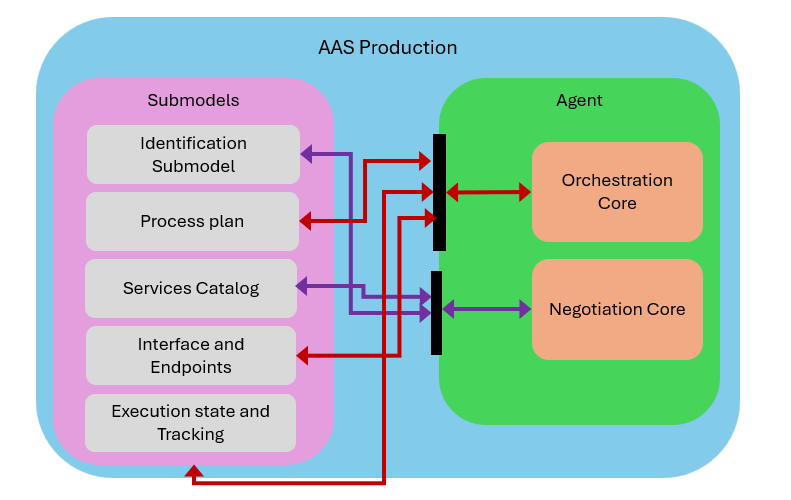
\includegraphics[width=0.9\textwidth]{Images/Production_Agent_overview.png}
    \caption{Product AAS Overview}
    \label{fig:product_aas_overview}
\end{figure}

\newpage
The Product AAS can interact with other AASs (production or resource).
It also capable of publishing events and subscribing to other AAS events.
As shown in figure \ref{fig:product_aas_interactions}, the Product AAS can interact with other AASs through
via XMPP protocol which is a communication protocol for MAS frame work for python \textbf{SPADE}.
XMPP can also be used as a broker for the AAS to publish and subscribe to events.
\begin{figure}[h]
    \centering
    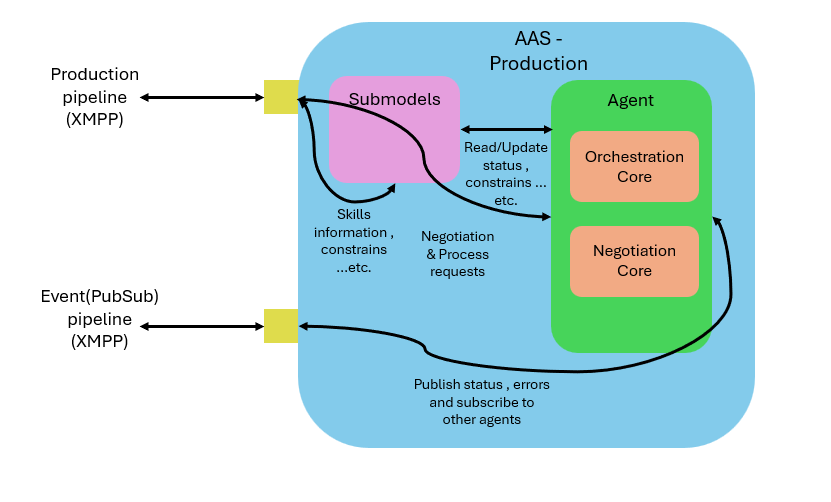
\includegraphics[width=0.99\textwidth]{Images/Production_Agent_Interaction_Overview.png}
    \caption{Product AAS Interactions - Overview}
    \label{fig:product_aas_interactions}
\end{figure}
The communication interfaces and their usage are summarized in table \ref{table:communication_interfaces_product}.
\begin{table}[h]
\centering
\begin{tabularx}{\textwidth}{>{\raggedright\arraybackslash}X>{\raggedright\arraybackslash}X}
\toprule
\rowcolor[HTML]{38FFF8}
\textbf{Communication Interface} & \textbf{Usage} \\ \midrule
XMPP & Agent-to-agent communication within the MAS framework. \\
XMPP - Events & Publishing and subscribing to events between AASs. \\
\bottomrule
\end{tabularx}
\caption{Communication Interfaces and Their Usage - Product AAS}
\label{table:communication_interfaces_product}
\end{table}
\newpage
Internally the Submodels are connected to the agent where they could be read and updated.
The Submodels can also provide the production agents with the process plan and the required services and skills
to perform the production process.
The Orchestration Core can manage the production process and coordinate the resources.
The Negotiation Core can communicate with other agents in the system via XMPP protocol.
The Negotiation Core can also register itself with a Agent Registry service that the Resource Agents
use for discovering the available products in the system.

\newpage
\subsubsection{Product AAS - Architecture Overview }

\begin{figure}[h]
    \centering
    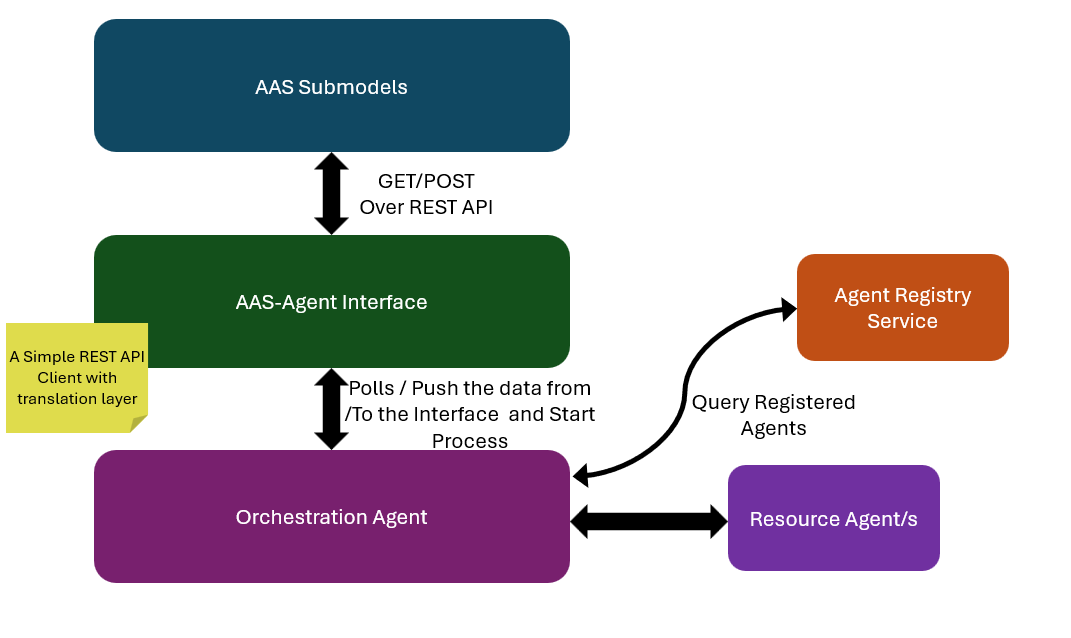
\includegraphics[width=0.99\textwidth]{Images/Production_Agent_Arch_overview.png}
    \caption{Product AAS Architecture Overview}
    \label{fig:product_aas_architecture_overview}
\end{figure}

From an Architecture point of view the Product AAS can be illustrated as in figure \ref{fig:product_aas_architecture_overview}.
The overview of the architecture shows three main layers, The \textbf{AAS Submodels} , \textbf{The AAS - Agent Interface} and Finally  \textbf{Orchestration Agent}.
The AAS Submodels layer are created via \textbf{Basyx} framework which is an open source framework for creating AASs.
This framework provides the necessary tools to create and manage AASs and their submodels.
It also can provide a REST API for the AAS to be accessed and managed.
The AAS - Agent Interface layer is responsible for connecting the AAS to the Orchestration Agent.
It mainly work as a middleman between the AAS and the Orchestration Agent where it translate the data types of from and to the AAS and the Orchestration Agent.
Finally The Orchestration Agent is the main component of the Product AAS where it contains the Orchestration Core and the Negotiation Core that represents the product in the system.
The Orchestration Core and the Negotiation Core are created via \textbf{SPADE} framework which is an open source framework for creating Multi-agent systems in python.
The Orchestration Core is responsible for managing the overall production process and coordinating the resources.
The Negotiation Core is responsible for negotiating with the Resource Agents to allocate the necessary resources for the production process.
The Orchestration Core and the Negotiation Core can also communicate with other agents in the system via XMPP protocol.
The Orchestration Core and the Negotiation Core also can register itself with a Agent Registry service that the Resource Agents
use for discovering the available products in the system.

\newpage
\subsubsubsection{Submodels with REST API and server}
\begin{figure}[h]
    \centering
    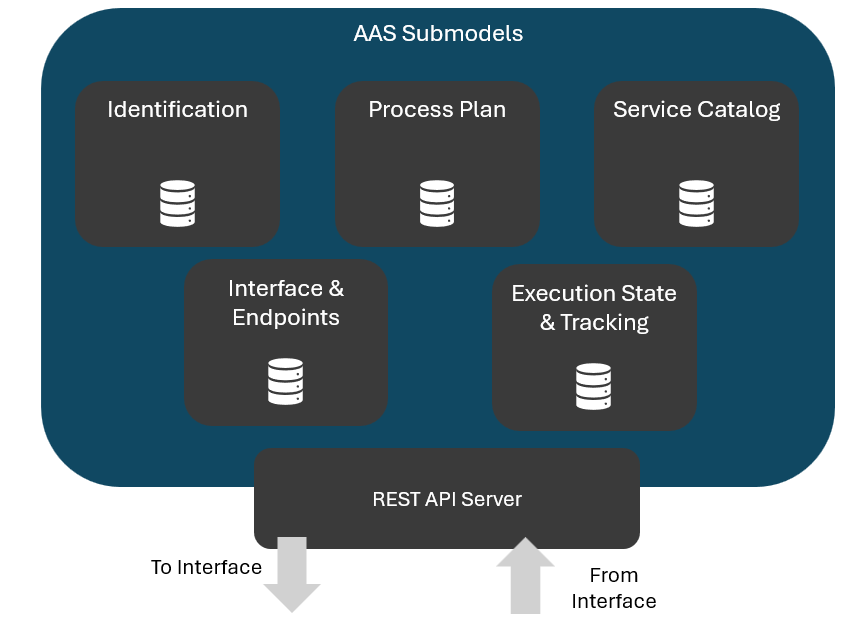
\includegraphics[width=0.8\textwidth]{Images/Production_Agent_Submodels_Arch_Overview.png}
    \caption{Product AAS Submodels with REST API and Server}
    \label{fig:product_aas_submodels_rest_api}
\end{figure}

Similar to the Resource AAS Submodels layer as shown in figure \ref{fig:product_aas_submodels_rest_api} contains the AAS Submodels and a REST API server.
The AAS Submodels are created via \textbf{Basyx} framework which is an open source framework for creating AASs.
This framework provides the necessary tools to create and manage AASs and their submodels.
It also can provide a REST API for the AAS to be accessed and managed.
The Submodels connects to the AAS-Agent Interface via REST API calls where the AAS-Agent Interface can read and update the submodels.

\newpage

\subsubsubsection{AAS-Agent Interface}

Similar to the Resource AAS-Agent Interface as in figure \ref{fig:resource_aas_agent_interface} the Product AAS-Agent Interface is responsible for connecting the AAS to the Orchestration Agent.
It mainly work as a middleman between the AAS and the Orchestration Agent where it translate the data types of from and to the AAS and the Orchestration Agent.
The main diffrence to the Resource AAS-Agent Interface is that it connects to the Orchestration Agent instead of the BDI Agent Core which means the data model to translate is diffrent.
\subsubsubsection{Orchestration Agent and Negotiation Core}

\begin{figure}[h]
    \centering
    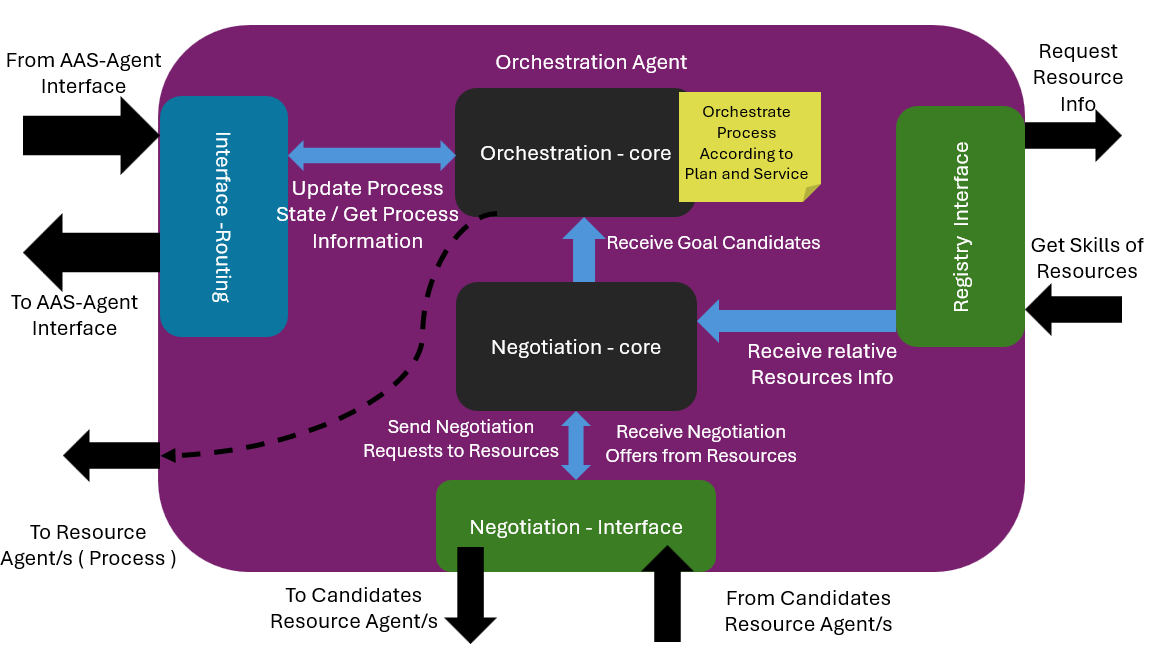
\includegraphics[width=0.99\textwidth]{Images/Production_Agent_Orchestration_Overview.png}
    \caption{Product AAS - Orchestration Agent and Negotiation Core}
    \label{fig:product_aas_orchestration_agent}
\end{figure}

As in figure \ref{fig:product_aas_orchestration_agent} the Orchestration Agent is the main component of the Product AAS where it contains the Orchestration Core and the Negotiation Core that represents the product in the system.
The Orchestration Core and the Negotiation Core are created via \textbf{SPADE} framework which is an open source framework for creating Multi-agent systems in python.
The Orchestration Core is responsible for managing the overall production process and coordinating the resources.
The Negotiation Core is responsible for negotiating with the Resource Agents to allocate the necessary resources for the production process.
The Orchestration Core and the Negotiation Core can also communicate with other agents in the system via XMPP protocol.

After landing a deal with the Resource Agents the Negotiation Core informs the Orchestration Core about the allocated resources.
The Orchestration Core then manages the production process using the allocated resources.
The Orchestration Core connects with the AAS-Agent Interface so that it can read and update the AAS Submodels.
The Orchestration Core also connects to other agents in the system via XMPP protocol.
The Orchestration Core can delegate tasks to the Negotiation Core so that it can focus on managing the production process.

The Negotiation Core also connects to the Registry Service so that it can discover the available Resource Agents in the system.
The Registry Service contains information about the available Resource Agents in the system including their capabilities and skills.
The Negotiation Core uses this information to negotiate with the Resource Agents to allocate the necessary resources for the production process.
